% CVPR 2023 Paper Template
% based on the CVPR template provided by Ming-Ming Cheng (https://github.com/MCG-NKU/CVPR_Template)
% modified and extended by Stefan Roth (stefan.roth@NOSPAMtu-darmstadt.de)

\documentclass[10pt,twocolumn,letterpaper]{article}

%%%%%%%%% PAPER TYPE  - PLEASE UPDATE FOR FINAL VERSION
\usepackage{cvpr}      % To produce the REVIEW version


% Include other packages here, before hyperref.
\usepackage{graphicx}
\usepackage{amsmath}
\usepackage{amssymb}
\usepackage{booktabs}


% It is strongly recommended to use hyperref, especially for the review version.
% hyperref with option pagebackref eases the reviewers' job.
% Please disable hyperref *only* if you encounter grave issues, e.g. with the
% file validation for the camera-ready version.
%
% If you comment hyperref and then uncomment it, you should delete
% ReviewTempalte.aux before re-running LaTeX.
% (Or just hit 'q' on the first LaTeX run, let it finish, and you
%  should be clear).
\usepackage[pagebackref,breaklinks,colorlinks]{hyperref}


% Support for easy cross-referencing
\usepackage[capitalize]{cleveref}
\crefname{section}{Sec.}{Secs.}
\Crefname{section}{Section}{Sections}
\Crefname{table}{Table}{Tables}
\crefname{table}{Tab.}{Tabs.}


%%%%%%%%% PAPER ID  - PLEASE UPDATE
\def\cvprPaperID{*****} % *** Enter the CVPR Paper ID here
\def\confName{CVPR}
\def\confYear{2023}

\begin{document}

%%%%%%%%% TITLE - PLEASE UPDATE
\title{Team \#16: Interim Report}

\author{
    Camilo Martínez\\
    7057573\\
    \and
    Dhimitrios Duka\\
    7059153\\
    \and
    Honglu Ma\\
    7055053\\
}
\maketitle

%%%%%%%%% BODY TEXT
\section{Progress Report}


\subsection{Creation of a custom dataset}
In the original paper, the authors train the models in a custom dataset that contains 14 classes (A, Am, B, Bm, C, Cm, D, Dm, E, Em, F, Fm, G, Gm). However, the datasets that we were able to find lacked some of them, mainly the minor chords. We employed two solutions to this problem. First, we enriched the dataset that we found by adding the missing classes. Second, we created our dataset. The setup was simple. First, a video for each chord was recorded using a smartphone. Each of the videos was 1:30 minutes long and was shot in 4k 60fps so that each retrieved frame would be of high quality and not subject to blurring. Second, we extracted each frame from the video and saved it as a downsampled image of size 640x360. In total, for each chord we had around 5000 frames, so we decided to use only 1 in 5 frames to reduce the overlap of the samples as much as possible. However, we still think that the sample overlapping could be an issue, so we will record more videos for each chord in the future.

\begin{figure*}[h]
    \begin{minipage}{0.45\textwidth}
        \centering
        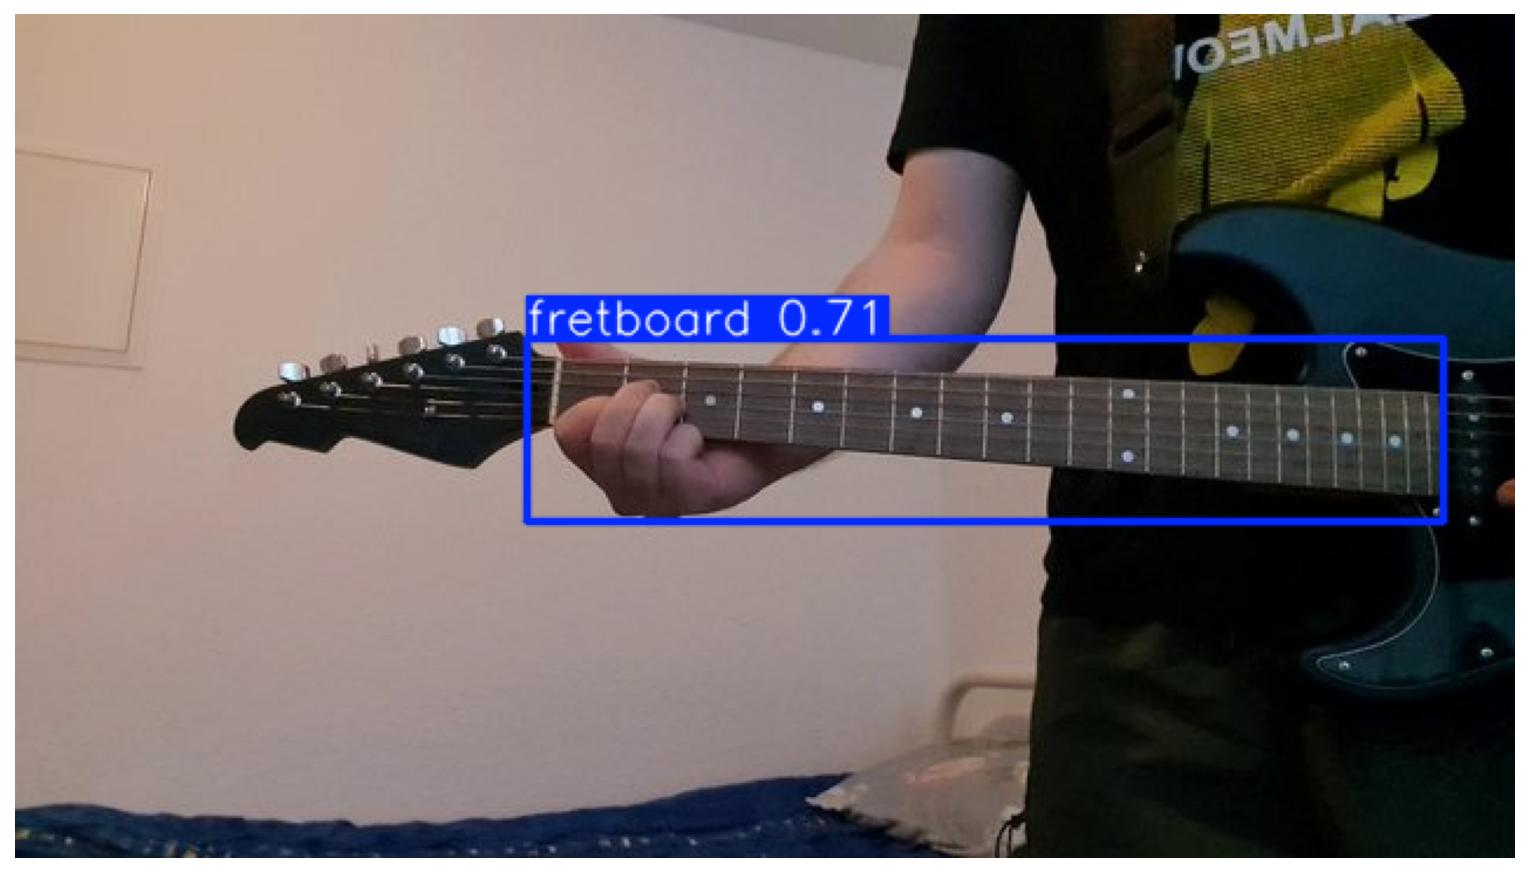
\includegraphics[width=\textwidth]{images/interim/dhimitrios-non-frozen.jpg}
    \end{minipage}
    \hfill
    \begin{minipage}{0.45\textwidth}
        \centering
        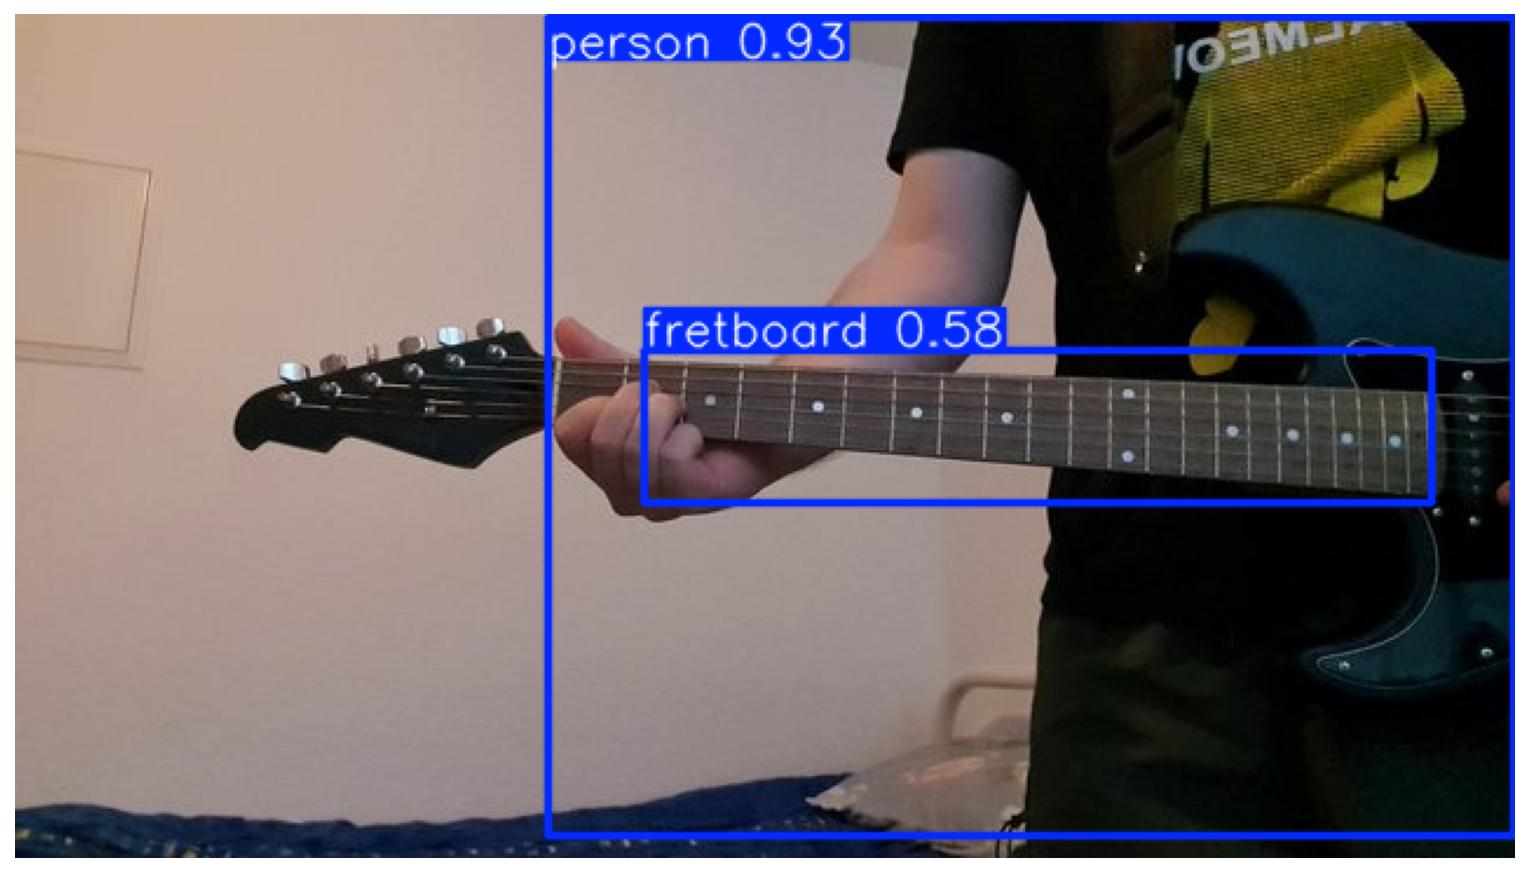
\includegraphics[width=\textwidth]{images/interim/dhimitrios.jpg}
    \end{minipage}
    \caption{\textbf{Left:} Prediction of our YOLOv9 \emph{fretboard detection model} finetuned without freezing the backbone. \textbf{Right:} Prediction of our YOLOv9 \emph{fretboard detection model} finetuned freezing every layer except the last one.}
    \label{fig:dataset-example}
\end{figure*}

\begin{figure*}[h]
    \begin{minipage}{0.33\textwidth}
        \centering
        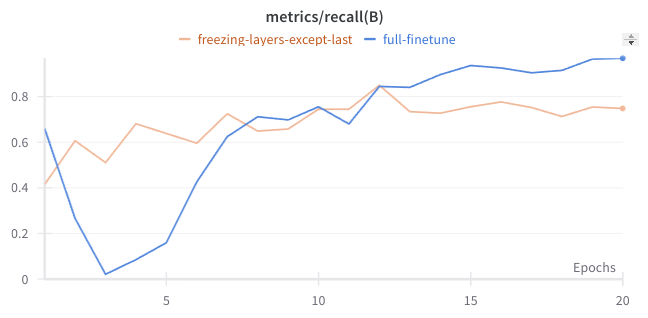
\includegraphics[width=\textwidth]{images/interim/metrics-recall-fretboard.png}
    \end{minipage}
    \hfill
    \begin{minipage}{0.33\textwidth}
        \centering
        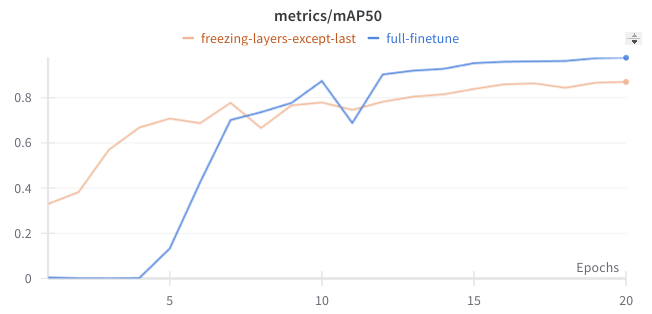
\includegraphics[width=\textwidth]{images/interim/metrics-mAP50-fretboard.png}
    \end{minipage}
    \hfill
    \begin{minipage}{0.33\textwidth}
        \centering
        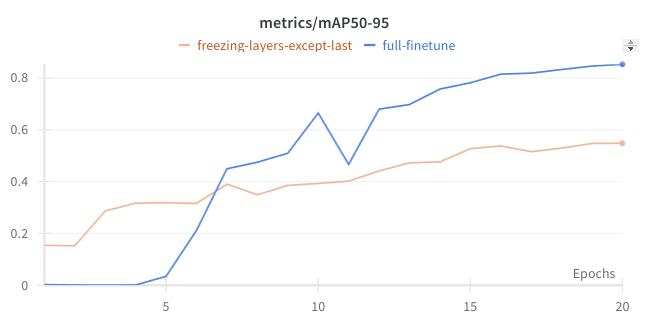
\includegraphics[width=\textwidth]{images/interim/metrics-mAP50-95-fretboard.png}
    \end{minipage}
    \caption{\textbf{Left:} Prediction of our YOLOv9 \emph{fretboard detection model} finetuned without freezing the backbone. \textbf{Right:} Prediction of our YOLOv9 \emph{fretboard detection model} finetuned freezing every layer except the last one.}
    \label{fig:metrics-fretboard}
\end{figure*}

\section{Fretboard Detection}


\section{Fine Tuning Visual Transformer (ViT)}
Different fine tuning methods were tried to adapt ViT to our inputs.
\subsection{Full Fine Tuning}
We first tried to fine tune the whole model. This was done by specifying the labels of our inputs to the pretrained model and it will attach a new MLP head to the classifier of the model which fits the dimensions of our labels and then the whole model were trained. We are getting a decent accuracy after adapting the model. \textbf{Attach figure of full fine tuning accuracy here.}

Next up, to be able to fine tune bigger models, we decided to try out other adaptation methods, especially the ones that reduce the trainable parameters of the model.

\subsection{Training only the MLP head}
We tried to train only the MLP head of the model. This was done by freezing the weights of the model and only training the weights of the classifier. However, this method was not successful and resulted in a bizarrely low accuracy. Our suspicion is that the pretrained model is not able to capture the features of our inputs and the extended MLP head is merely trying to predicting the labels on its own i.e. the same as a feed forward network.
We also tried to unfreeze more layers of the model and they also didn't meet the expectation but the accuracy did increase which sorts of confirms our suspicion.
\subsection{LoRA}
To let the model extract useful features from our inputs, we cannot risk to freeze the encoders completely. Our next attempt was to use the low rank adaptation (LoRA) method. It is a method that reduces the number of parameters of the model by factorizing the weights of the projections in the attention part of the model. In this way, we hope to let the feature learned by the model and also decrease the number of trainable parameters. We are still in the process of trying this method and we are expecting to see some improvements in the accuracy.

\section{Problems Encountered}
We encountered several issues during our work. Firstly, we faced some problems with the cluster. At first, we could not configure a conda environment or run our code. After some debugging, we were able to solve the problem by installing the packages in chunks instead of all at once.

Second, we faced some problems while fine-tuning YOLOv9 for fretboard detection. At first, we were using Ultralytics to fine-tune the model. However, we noticed that the final model recognized only two classes: the fretboard and the background. This meant that the model was forgetting all other classes on which it was trained. We addressed this problem by implementing another approach based on \cite{}.

Lastly, during the classification phase, we faced some problems with data leakage. We noticed a rather high classification accuracy of 99\% in the validation set which was surprising to us. After some debugging, we found out that the problem originated from the preprocessing that we had applied to our classification dataset.


    %%%%%%%%% REFERENCES
    {\small
        \bibliographystyle{ieee_fullname}
        \bibliography{references}
    }

\end{document}
